\documentclass{article}
\usepackage[utf8]{inputenc}
\usepackage{polski}
\usepackage{geometry}
\usepackage{pdfpages}
\usepackage{pdfpages}
\usepackage{listings}
\usepackage{listingsutf8}
\usepackage{multirow}
\usepackage{siunitx}
\usepackage{multirow}
\usepackage{booktabs}
\usepackage{tabularx}
\usepackage{placeins}
\usepackage{pdflscape}
\usepackage{colortbl}

\geometry{
a4paper,
total={170mm,257mm},
left=20mm,
top=20mm
}
\newcolumntype{Y}{>{\centering\arraybackslash}X}
% \renewcommand\thesection{}
\lstset{%
literate=%
 {ą}{{\k{a}}}1
 {ę}{{\k{e}}}1
 {Ą}{{\k{A}}}1
 {Ę}{{\k{E}}}1
 {ś}{{\'{s}}}1
 {Ś}{{\'{S}}}1
 {ź}{{\'{z}}}1
 {Ź}{{\'{Z}}}1
 {ń}{{\'{n}}}1
 {Ń}{{\'{N}}}1
 {ć}{{\'{c}}}1
 {Ć}{{\'{C}}}1
 {ó}{{\'{o}}}1
 {Ó}{{\'{O}}}1
 {ż}{{\.{z}}}1
 {Ż}{{\.{Z}}}1
 {ł}{{\l{}}}1
 {Ł}{{\l{}}}1
}

\title{Technika Cyfrowa\\
Sprawozdanie - Przerzutniki i rejestry}
\author{Maciej Trątnowiecki}
\date{AGH, Semestr Letni, 2020}

\begin{document}
    \maketitle
    \section{Projekt przerzutnika RS}
        \subsection{Projekt układu}
            Przypomnijmy tabelę prawdy przerzutnika RS.
            \begin{center}
                \begin{table}[ht]
                    \centering
                    \begin{tabular}{|c|c|c|c|}
                        \hline
                        S & R & $Q_n$ & $\neg$ Q\\
                        \specialrule{1pt}{1pt}{1pt}
                        0 & 0 & $Q_{n-1}$  & $\neg Q_{n-1}$\\
                        \hline
                        1 & 0 & 1 & 0\\
                        \hline
                        0 & 1 & 0 & 1\\
                        \hline
                        1 & 1 & - & -\\
                        \hline 
                    \end{tabular}
                    \caption{Tabela prawdy przerzutnika RS}
                    \label{tab:my_label}
                \end{table}
            \end{center}
            Gdy zarówno wejście S jak i R otrzyma stan niski, chcemy żeby nasz układ nie zmienił stanu podanego na wyjście. Zauważmy, że jest to równoważne z negację stanu wyjścia zanegowanego. Bramka NOR neguje stan podany na jedno z wejść, jeśli na drugim wejściu jest podany stan niski.\\
            Jeśli na wejście S podamy stan wysoki, a na wejście R stan niski, chcemy otrzymać stan wysoki na wyjściu układu. Bramka NOR poda zawsze stan niski, gdy otrzyma stan wysoki na którymkolwiek z wejść. Otrzymujemy zatem zależności: 
            \begin{itemize}
                \item Stan niski na obu z wejść - na każdym z dwóch wyjść podajemy negację stanu drugiego wyjścia/
                \item Stan niski na wejściu R i wysoki na S - Na wyjściu zanegowanym podajmy stan niski, na wyjściu Q negację drugiego wyjścia. 
                \item Stan niski na wejściu S i wysoki na R - Na wyjściu Q podajemy stan niski, na drugim negację wyjścia Q.
            \end{itemize}
            \FloatBarrier
            Do budowy układu zachowującego się w sposób opisany powyżej wystarczą nam dwie bramki NOR. Ich wyjścia połączymy z wyjściami układu. Jedno z wejść każdej z bramek połączone będzie z odpowiednim wejściem układu, drugie z wyjściem drugiej bramki. 

            \begin{center}
                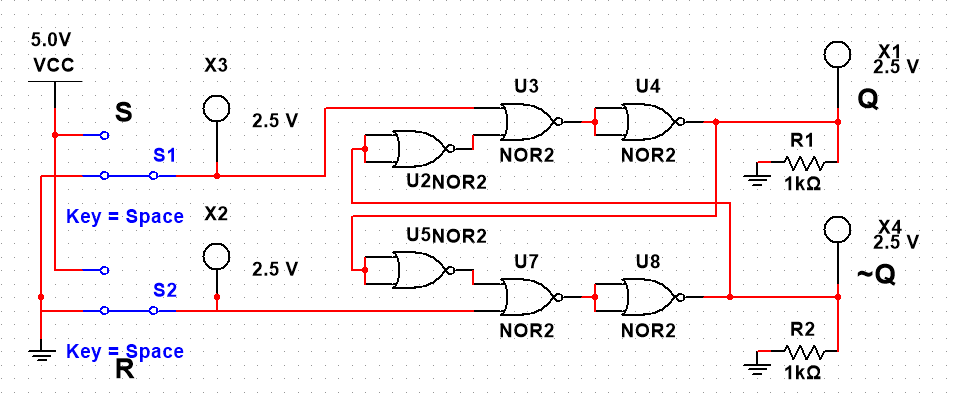
\includegraphics[width=18cm]{reports/img/Z2A_1.png}\\
            \end{center}
            Układ realizuje funkcje opisaną poniższą tabelą prawdy. Układ przetestowałem z wykorzystaniem próbówek, weryfikując stan wyjść układu dla każdej z trzech konfiguracji wejść. Otrzymałem odczyty zgodne z zakładaną tabelą prawdy przerzutnika, wykazując że układ funkcjonuje poprawnie. 
        
        \subsection{Wnioski}
            Udało nam się pokazać, że układ przerzutnika RS można łatwo skonstruować przy użyciu prostych i powszechnie dostępnych bramek logicznych. 
        
    \section{Budowa przerzutnika T}
        \subsection{Projekt układu}
            Ponieważ w konstrukcji przerzutnika chcemy wykorzystać przerzutnik RS, zestawmy tabele prawdy przerzutnika T ze stanami wejść przerzutnika RS dla odpowiadających im wartości wyjść. 
            \begin{center}
                \begin{table}[ht]
                    \centering
                    \begin{tabular}{|c|c|c|c|c|}
                        \hline
                        T & $Q_n$ & $Q_{n+1}$ & S & R\\
                        \specialrule{1pt}{1pt}{1pt}
                        0 & \cellcolor{green!40}0 & \cellcolor{orange!40}0 & \cellcolor{orange!40}0 &\cellcolor{green!40} 0 \\
                        \hline
                        0 &\cellcolor{green!40} 1 & \cellcolor{orange!40} 1 &\cellcolor{orange!40} 0 &\cellcolor{green!40} 0\\
                        \hline
                        1 &\cellcolor{green!40} 0 & \cellcolor{orange!40}1 &\cellcolor{orange!40} 1 &\cellcolor{green!40} 0\\
                        \hline
                        1 &\cellcolor{green!40} 1 &\cellcolor{orange!40} 0 &\cellcolor{orange!40}\cellcolor{orange!40} 0 &\cellcolor{green!40} 1\\
                        \hline 
                    \end{tabular}
                    \caption{Tabela prawdy przerzutnika T z odpowiadającymi jej stanami wejść przerzutnika RS}
                    \label{tab:my_label}
                \end{table}
            \end{center}
            Będziemy chcieli dobrać funkcje logiczne opisujące zależność pomiędzy stanem wyjść układu przerzutnika RS, oraz wejścia T, a wejściami R i S. \\
            Zauważmy, że taką zależność możemy uzyskać za pomocą dwóch bramek AND. Wartość na wejściu S opiszemy jako koniunkcję logiczną wejścia T i wyjścia zanegowanego Q. Z kolei wartość na wejściu R opiszemy jako koniunkcję logiczną wejścia T z wyjściem Q.\\
            W efekcie uzyskujemy poniższy układ.
            \begin{center}
                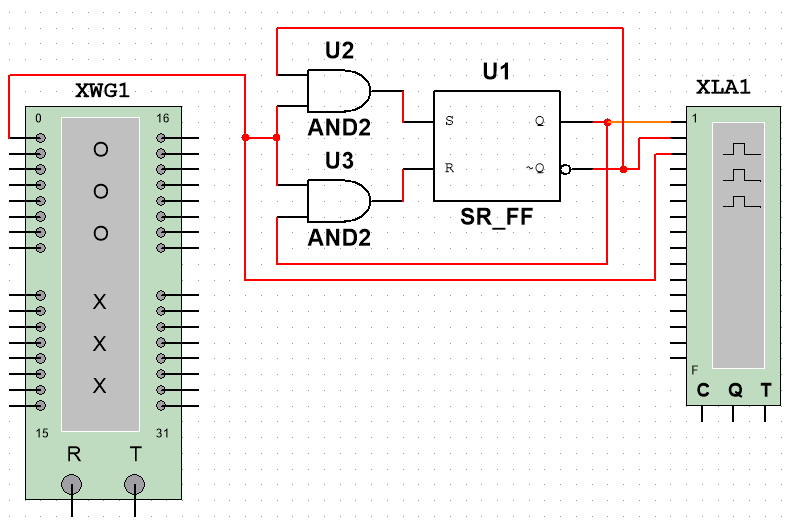
\includegraphics[width=18cm]{reports/img/Z2B_1.png}\\
            \end{center}
            
            \subsection{Sposób działania układu}
            Przerzutnik T posiada jedno wejście - T i dwa wyjścia - Q i zanegowane Q. Do wejścia T przerzutnika podłączyłem generator słów. Do wyjść przerzutnika podłączyłem analizator logiczny.\\ 
            Przerzutnik T realizuje funkcję opisaną poniższą tabelą stanów. 
            \begin{center}
                \begin{table}[ht]
                    \centering
                    \begin{tabular}{|c|c|c|}
                        \hline
                        T & $Q_n$ & $Q_{n+1}$\\
                        \specialrule{1pt}{1pt}{1pt}
                        0 & 0 & 0\\
                        \hline
                        0 & 1 & 1\\
                        \hline
                        1 & 0 & 1\\
                        \hline
                        1 & 1 & 0\\
                        \hline 
                    \end{tabular}
                    \caption{Tabela prawdy przerzutnika T}
                    \label{tab:my_label}
                \end{table}
            \end{center}
            Co potwierdziłem za pomocą analizatora, otrzymując poniższe wyniki.
            \begin{center}
                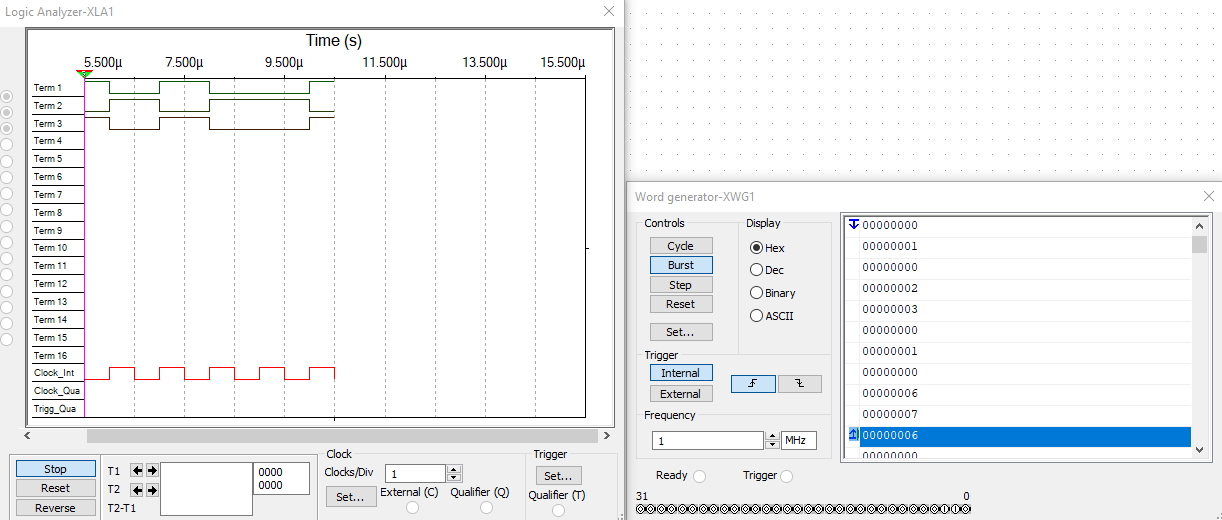
\includegraphics[width=18cm]{reports/img/Z2B_2.png}\\
            \end{center}

            
        \subsection{Wnioski}
            Przy użyciu prostych bramek logicznych możemy przeprowadzać konwersję pomiędzy poszczególnymi typami przerzutników. Zestawiając ich wyjścia możemy w prosty sposób wyprowadzić odpowiednie zależności umożliwiające konwersję. 
    
    \section{Układ szeregowy nadajnika - odbiornika}
        \subsection{Projekt układu}
            \begin{center}
                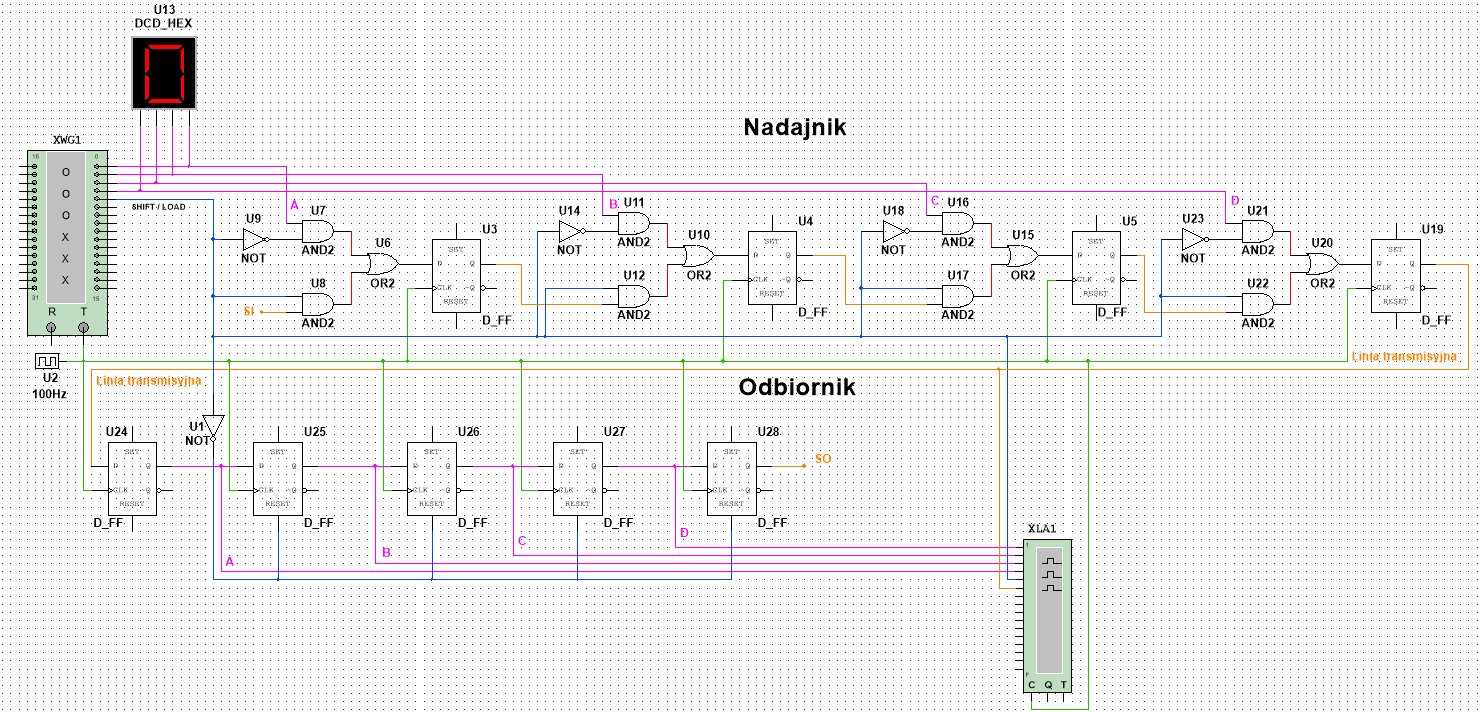
\includegraphics[width=18cm]{reports/img/Z2C_1.png}\\
            \end{center}
            Rejestry nadajnika i odbiornika zbudowałem z wykorzystaniem przerzutników D. Generator słów podaje na wejście układu nadajnika czterobitową liczbę (jako sygnał równoległy). Nadajnik przekazuje liczbę jako sygnał szeregowy. Układ odbiornika odczytuje sygnał szeregowy do sygnału równoległego. Jego wyjścia połączone są z analizatorem logicznym. Za przesunięcie liczby przez rejestry odpowiednią ilość razy odpowiada układ zbudowany z użyciem licznika modulo i bramek logicznych umieszczony w lewym dolnym rogu płytki. 
            
        \subsection{Sposób działania układu}
            Wejście układu, postaci czterobitowej liczby w formacie równoległym zostaje przekazane do rejestru PISO. Sygnał shift ustawiony jest w stan niski. Stany odpowiadające za kolejne bity liczby wejściowej przekazane zostają na wejścia D odpowiadających im przerzutników D. Następnie sygnał shift ustawiony zostaje w stan wysoki. Przez cztery kolejne okresy zegara stany odpowiadające za kolejne bity liczby wejściowej zostają "przesunięte", tj. przekazane przez linię sygnału szeregowego do odbiornika. Stan przekazany w początkowej fazie do przerzutnika przesuwany jest do kolejnego przerzutnika, by w końcu trafić na linię transmisyjną.  Możliwe jest to dzięki wykorzystaniu przerzutników D kopiujących stan wejścia na wyjścia po otrzymaniu sygnału zegarowego, oraz użytych przed wejściami bramek logicznych. Przełączają one wejście pomiędzy poprzednią bramką i generatorem w zależności od stanu wejścia shift. \\
            
            Z linii transmisyjnej sygnał szeregowy trafia do rejestru SIPO, który przetwarza go do formatu równoległego. Sygnał szeregowy trafia na wejście przerzutnika D. Wyjście przerzutnika do połączone jest z kolejnym przerzutnikiem. Za wyjściami przerzutników podłączamy kolejne wyjścia sygnału równoległego. Po wykonaniu odpowiednią ilość razy przesunięcia, wyjścia równoległe poprawnie reprezentują transmitowaną liczbę. \\
            
            \begin{center}
                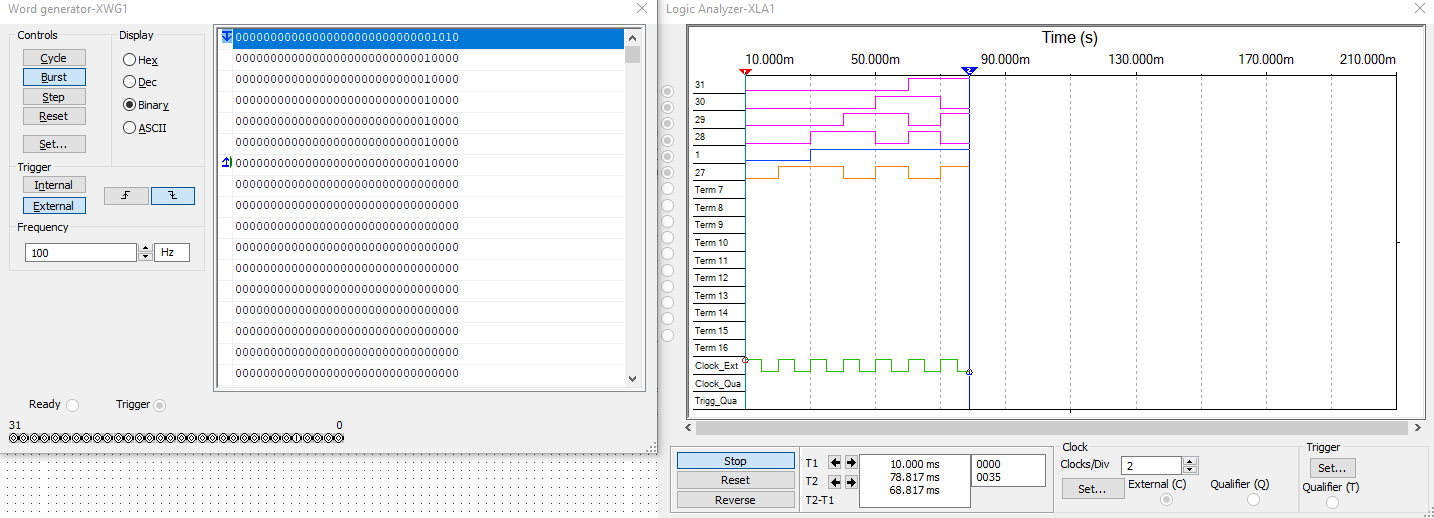
\includegraphics[width=18cm]{reports/img/Z2C_2.png}\\
            \end{center}
            Układ przetestowany został z użyciem analizatora logicznego, wykazując oczekiwaną częstotliwość sygnału shift i poprawność przesłanych danych. Widzimy, że udało nam się przesłać liczbę czterobitową, za pomocą pojedynczej linii transmisyjnej. 
            
        \subsection{Wnioski}
            Przy użyciu podstawowych przerzutników zbudować możemy rejestry realizujące konwersję danych z komunikacji szeregowej na równoległą. Pozwala to na budowę wydajniejszych systemów komunikacyjnych pomiędzy poszczególnymi układami cyfrowymi. 

\end{document}
